
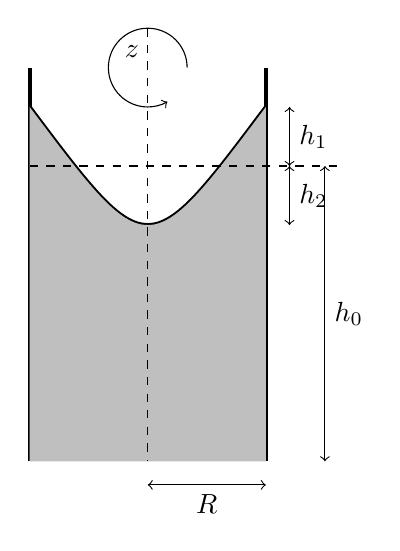
\begin{tikzpicture}

    % Cylinder walls
    \draw[line width=0.5mm] (-1.5,0) -- (-1.5,5);
    \draw[line width=0.5mm] (1.5,0) -- (1.5,5);

    % Curved liquid surface
    \draw[line width=0.5mm] (-1.5,4.5) .. controls (0,2.5) and (0,2.5) .. (1.5,4.5);
    
    % Shaded liquid area
    \fill[gray!50] (-1.5,0) -- (-1.5,4.5) .. controls (0,2.5) and (0,2.5) .. (1.5,4.5) -- (1.5,0) -- cycle;
    
    % Vertical center line
    \draw[dashed] (0,5.5) -- (0,0);
    \draw[dashed] (-1.5,3.75) -- (2.5,3.75);

    % Rotation arrow in the middle
    \draw[->] (0.5,5) arc[start angle=0, end angle=300, radius=0.5] ;

    % Labels for heights and radius
    \draw[<->] (1.8,3.75) -- (1.8,4.5) node[midway,right] {$h_1$};
    \draw[<->] (1.8,3) -- (1.8,3.75) node[midway,right] {$h_2$};
    \draw[<->] (2.25,0) -- (2.25,3.75) node[midway,right] {$h_0$};
    
    % Radius label
    \draw[<->] (0, -0.3) -- (1.5, -0.3) node[midway, below] {$R$};

    % Axis labels
    \node at (-0.2,5.2) {$z$};
    
\end{tikzpicture}

